\documentclass{article}
\usepackage{arxiv}
\usepackage{wrapfig}
\usepackage{amsmath}
\usepackage[utf8]{inputenc}
\usepackage[english, russian]{babel}
\usepackage[T1]{fontenc}
\usepackage{url}
\usepackage{booktabs}
\usepackage{float}
\usepackage{amsfonts}
\usepackage{diagbox}
\usepackage{nicefrac}
\usepackage{microtype}
\usepackage{lipsum}
\usepackage{amssymb}
\usepackage{graphicx}
\usepackage{natbib}
\usepackage{doi}
\usepackage{makecell}

\pagestyle{fancy}



\title{Восстановление значения многомерного временного ряда в точке по спрогнозированной матрице попарных корреляций}

\author{ Maxim Divilkovskiy \\
% \thanks{Use footnote for providing further
% 		information about author (webpage, alternative
% 		address)---\emph{not} for acknowledging funding agencies.} \\
	Chair of Data Analysis\\
	MIPT\\
	\texttt{divilkovskii.mm@phystech.edu} \\
	%% examples of more authors
	\And
	Vadim Strijov \\
	FRC CSC of the RAS\\
	Moscow, Russia\\
    \texttt{strijov@phystech.edu} \\
    \And
    Konstantin Yakovlev \\
    Chair of Intellectual Systems\\
    MIPT\\
    \texttt{iakovlev.kd@phystech.edu} \\
	% Santa Narimana, Levand \\
	% \texttt{stariate@ee.mount-sheikh.edu} \\
	%% \AND
	%% Coauthor \\
	%% Affiliation \\
	%% Address \\
	%% \texttt{email} \\
	%% \And
	%% Coauthor \\
	%% Affiliation \\
	%% Address \\
	%% \texttt{email} \\
	%% \And
	%% Coauthor \\
	%% Affiliation \\
	%% Address \\
	%% \texttt{email} \\
}
\date{}

\renewcommand{\shorttitle}{\textit{arXiv} Template}

%%% Add PDF metadata to help others organize their library
%%% Once the PDF is generated, you can check the metadata with
%%% $ pdfinfo template.pdf
\hypersetup{
pdfauthor={Maxim Divilkovskiy},
}

\graphicspath{ {./figures/} }

\begin{document}
\maketitle

\begin{abstract}
	Решается задача поточечного прогнозирования набора временных рядов с высокой ковариацией и высокой дисперсией. Для решения данной задачи предлагается построить пространство парных расстояний. В этом пространстве прогнозируется матрица попарных расстояний, а затем по известной матрице восстанавливаются значения временных рядов.
	В данной статье изучается способ восстановления прогноза в пространстве временных рядов по известной матрице попарных расстояний. Показывается существование нескольких значений временного ряда, удовлетворяющих одной матрице попарных расстояний. Предлагается несколько алгоритмов, основанных на использовании матриц, построенных по различным временным интервалам с использованием попарной корреляции. Так же, в статье выводится явный вид восстановленных значений через матрицу попарных корреляций. Помимо этого, приводится оценка качества восстановления при добавлении шума в матрицы попарных расстояний. Новизна метода заключается в том, что прогнозирование делается не в исходном пространстве, а в пространстве попарных расстояний.


\end{abstract}


\keywords{Metric \and Non-Convex Optimization \and Correlation \and Time Series Forecasting}

\section{Введение}
	Цель данной работы заключается в представлении нового метода поточечного прогнозирования временных рядов. Рассматриваемые ряды характеризуются высокой попарной ковариацией и высокой дисперсией. Задача поточечного прогнозирования заключается в вычислении значений временных рядов в следующий момент времени по имеющимся историческим данным за предыдущие несколько моментов. Задача разбивается на три этапа: сначала исходное пространство временных рядов трансформируется в метрическое пространство при помощи построения матрицы попарных расстояний. Затем в этом пространстве осуществляется прогноз матрицы попарных расстояний в следующий момент времени. В теоретической части статьи показана необходимость прогноза не менее чем двух матриц. Показывается, что для единственности ответа требуется использовать несколько матриц, отвечающих различным временным интервалам. Последним этапом, по спрогнозированным матрицам результат возвращается в исходное пространство. Статья фокусируется в первую очередь на последнем этапе. Приводятся эксперименты в случае с точным прогнозом матрицы с добавлением к значениям нормального шума.
		
	Существующие способы предсказания временных рядов, такие как LSTM \cite{LSTM}, SSA \cite{SSA} и другие \cite{Biosignals}, \cite{boyd2017multiperiod} основаны на предсказании значения одного ряда. При этом, данные методы могут быть изменены для прогноза в том числе набора временных рядов. Для этого достаточно рассматривать набор рядов как один многомерный ряд. Однако, такой подход не моделирует в явном виде зависимости между различными рядами. В данной работе предлагается анализировать изменение \textit{набора} временных рядов. В таком подходе явно используются связи между ними в качестве информации. Подобное исследование проводится в статье \cite{MulticorrelatedQuadratic}, однако в ней делается упор на задаче feature selection. Данная задача заключается в выборе такого поднабора из исходных временных рядов, для которых возможно делать прогноз достаточного качества.
	
	В данной работе прогнозирование делается не в исходном пространстве, а в пространстве попарных расстояний. Преимущество данного метода заключается в том, что в реальных наборах временных рядов (природных, физических, финансовых и т.д.), часто наблюдается зависимость, близкая к линейной. Эта дополнительная информация способна улучшить качество итогового прогноза.
	
	Далее рассматриваюся условия на функцию расстояния между рядами при которых существует способ восстановления значений временных рядов. Доказывается недостаточность одной матрицы для восстановления ответа. Предлагается два метода, использующие несколько матриц, для случая точного прогноза и для случая прогноза с погрешностью. Так же предлагается алгоритм восстановления, основанный на двух теоремах о явном виде ответа при использовании попарной корреляции в качестве функции попарного расстояния между рядами. В качестве критериев качества используются MSE и MAE. В статье \cite{jadon2022comprehensive} показано, что они являются наиболее подходящими для задачи прогнозирования временных рядов.

\section{Постановка задачи поточечного прогнозирования набора временных рядов}

Набор из $d$ временных рядов задан $t$ векторами:

$$[\mathbf{x}_1, \mathbf{x}_2, \ldots, \mathbf{x}_t], \text{для всех } k: \mathbf{x}_k \in \mathbb{R}^d, $$

$\mathbf{x}_{t_i, k} \in \mathbb{R}$ задаёт собой значение ряда с индексом $k$ в момент времени $t_i$.

Задача заключается в прогнозе $\mathbf{x}_{t+1}$~--- набора значений всех временных рядов в момент времени $t+1$.

Матрица $\mathbf{x}$ размера $t \times d$ рассматривается как \textit{многомерный} временной ряд, рассматривая значение в точке как элемент пространства $\mathbb{R}^d$.

Ошибки предсказания вычисляются по следующим формулам:
\[
\text{MAE} = \frac{\sum_{i=1}^{d} |\mathbf{x_{t+1}} - \mathbf{\hat{x}_{t+1}}|}{d},
\]

\[
\text{MSE} = \frac{\sum_{i=1}^{d} (\mathbf{x_{t+1}} - \mathbf{\hat{x}_{t+1}})^2}{d}.
\]

\section{Общий вид алгоритма при прогнозе одной матрицы расстояний}

1. Строятся матрицы расстояний между набором значений временных рядов по нижеприведённой схеме.

\begin{align*}
	[\mathbf{x}_1, \ldots, \mathbf{x}_s] &\rightarrow \mathbf{\Sigma}_s \\
	[\mathbf{x}_2, \ldots, \mathbf{x}_{s+1}] &\rightarrow \mathbf{\Sigma}_{s+1} \\
	&\vdots \\
	[\mathbf{x}_{t-s}, \ldots, \mathbf{x}_t] &\rightarrow \mathbf{\Sigma}_{t}
\end{align*}

Все $\mathbf{\Sigma}_i$~--- матрицы попарных расстояний размера $d \times d$. Элемент матрицы $\mathbf{\Sigma}_{i,j}$ является значением расстояния между рядами $i$ и $j$. Формула построения, так же как и выбор функции расстояния описаны в следующих секциях.

2. По этим матрицам прогнозируется матрица $\hat{\mathbf{\Sigma}}_{t+1}$

3. Находится такой $\mathbf{\hat{x}}_{t+1}$, что \[ ||\hat{\mathbf{\Sigma}}_{t+1} - \bar{\mathbf{\Sigma}}_{t+1}||_2^2 \] минимальна, где $\bar{\mathbf{\Sigma}}_{t+1}$~--- матрица расстояний, построенная по набору $[\mathbf{x}_{t-s+1}, \ldots, \mathbf{x}_{t}, \mathbf{\hat{x}}_{t+1}]$. Достижение минимума этой функцией будет означать равенство $\hat{\mathbf{\Sigma}}_{t+1}$ и $\bar{\mathbf{\Sigma}}_{t+1}$. В свою очередь это означает что найденное продолжение ряда на момент времени $t+1$ имеет матрицу расстояний, равную прогнозу. В общем случае, данная функция невыпуклая и минимумов может быть несколько.

\section{Существование нескольких значений ряда, удовлетворяющих одной матрице расстояний}

Существование нескольких решений задачи минимизации, описанной выше, является центральной проблемой, рассматриваемой в данной статье. В данной секции показывается, что по одной матрице, построенной по произвольной метрике, можно восстановить несколько различных значений рядов в следующий момент времени.

Рассматривается возвращение прогноза из матрицы $\mathbf{\Sigma}_{t+1}$ в пространство временных рядов, где $\mathbf{\Sigma}_{t+1}$ есть матрица попарных расстояний, отвечающая многомерному ряду $\mathbf{x}=[\mathbf{x_1}, \ldots, \mathbf{x_{t+1}}]$.

Дана матрица попарных расстояний $\mathbf{\Sigma}$ размера $d \times d$ для многомерного временного ряда $\mathbf{x} \in \mathbb{R}^{d \times (t+1)}$. Предсказывается $\hat{\mathbf{x}}_{t+1} \in \mathbb{R}^d$. Так же, известна метрика \[ d : \mathbb{R}^{t+1} \times \mathbb{R}^{t+1} \rightarrow \mathbb{R}, \] введённая на временных рядах, обладающая свойствами метрики. То есть, \[\mathbf{\Sigma}_{i,j} = d(\mathbf{x}_{1 \ldots t, i} \circ \hat{\mathbf{x}}_{t+1, i}, \mathbf{x}_{1 \ldots t, j} \circ \hat{\mathbf{x}}_{t+1, j}),\] где $\circ$ означает конкатенацию векторов.

Одной из часто используемых метрик является евклидова метрика. На её примере покажем, что подходящих ответов может быть несколько. Более того, в случае евклидовой метрики, ответов бесконечное количество.

\[\mathbf{\Sigma}_{i,j} = d(\mathbf{x}_{1 \ldots t, i} \circ \hat{\mathbf{x}}_{t+1, i}, \mathbf{x}_{1 \ldots t, j} \circ \hat{\mathbf{x}}_{t+1, j})=\sqrt{\left(\sum_{k=1}^t (\mathbf{x}_{k,i}-\mathbf{x}_{k,j})^2\right) + (\hat{\mathbf{x}}_{t+1, i}-\hat{\mathbf{x}}_{t+1, j})^2}.\]

Использование данной метрики приводит к тому, что прибавление ко всем $\hat{\mathbf{x}}_{t+1, i}$ некоторой константы $C$ не изменяет ответ:
\[
\sqrt{\left(\sum_{k=1}^t (\mathbf{x}_{k,i}-\mathbf{x}_{k,j})^2\right) + (\hat{\mathbf{x}}_{t+1, i}-\hat{\mathbf{x}}_{t+1, j})^2} = \sqrt{\left(\sum_{k=1}^t (\mathbf{x}_{k,i}-\mathbf{x}_{k,j})^2\right) + [(\hat{\mathbf{x}}_{t+1, i} + C) -(\hat{\mathbf{x}}_{t+1, j} + C)]^2}.
\]
В случае задачи предсказывания временных рядов это свойство критично, поскольку даже при точном предсказании матрицы $\mathbf{\Sigma}$ существует бесконечно много значений временных рядов в момент времени $t+1$, отвечающих этой матрице.

\begin{figure}[H]
	\centering
	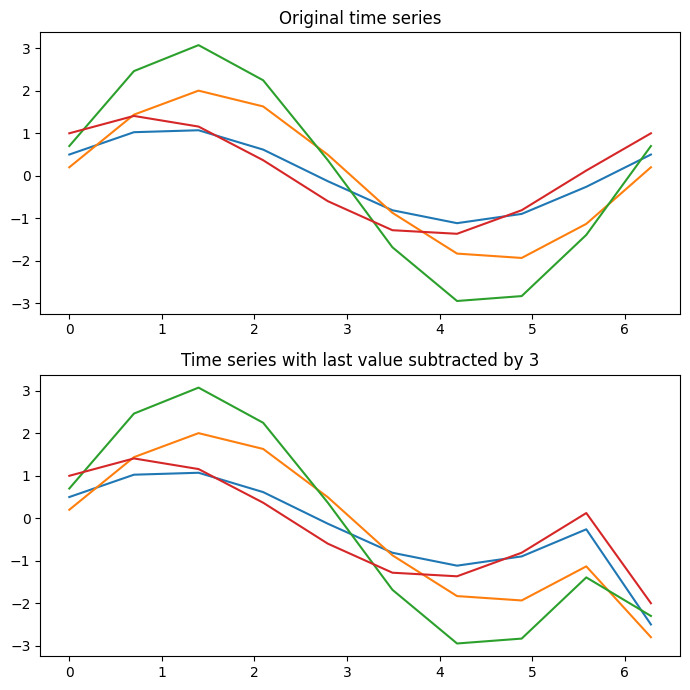
\includegraphics[width=\textwidth]{SameMatrix.jpg}
	\label{fig:fig1}
	\caption{Данные наборы временных рядов имеют одинаковую матрицу расстояний, построенную по евклидовой метрике.}
\end{figure}

Это приводит к невозможности использования алгоритма MDS для восстановления ответа в исходное пространство временных рядов.

Однако, даже использование других метрик не позволяет избавиться от проблемы.

\textbf{Теорема 1.} \textit{Для любой метрики, введённой в пространстве временных рядов $\mathbb{R}^t$, существует более одного способа восстановить исходные временные ряды из построенной по данной метрике матрице попарных расстояний.}

\textbf{Замечание.} В данном утверждении не используется информация о первых $t-1$ значениях ряда. В сущности, ряд в данном случае можно рассматривать в качестве точки в пространстве $\mathbb{R}^t$. Использование информации о предыдущих моментах времени приведено после данной теоремы.

\textbf{Доказательство.} Достаточно показать, что метрика не является биекцией. Это будет означать, что существуют несколько различных пар рядов, расстояние между которыми одинаковое.

Покажем, что метрика~--- непрерывная функция. Возьмём последовательность \[\{(\mathbf{x}_n, \mathbf{y}_n)\} \subset \mathbb{R}^t \times \mathbb{R}^t, (\mathbf{x}_n, \mathbf{y}_n) \to (\mathbf{x}, \mathbf{y}).\] Тогда, \[\mathbf{x}_n\to \mathbf{x}, \mathbf{y}_n\to \mathbf{y} \Rightarrow d(\mathbf{x}_n,\mathbf{x})\to 0 ,d(\mathbf{y}_n,\mathbf{y})\to 0,\] $при n \to \infty.$ Воспользовавшись неравенством треугольника для метрики, получаем \[d(\mathbf{x}_n,\mathbf{y}_n)\leqslant d(\mathbf{x}_n,\mathbf{x})+d(\mathbf{x},\mathbf{y})+d(\mathbf{y}_n,\mathbf{y})\to d(\mathbf{x},\mathbf{y}),\] следовательно, $d(\mathbf{x}_n,\mathbf{y}_n)\to d(\mathbf{x},\mathbf{y})$.

То есть метрика~--- непрерывное отображение из $\mathbb{R}^t \times \mathbb{R}^t$ в $\mathbb{R}$. Покажем, что такое отображение не может быть гомеоморфизмом. Предположим, что $f: \mathbb{R} \to \mathbb{R}^t \times \mathbb{R}^t$~--- искомый гомеоморфизм. Возьмём некоторую точку $a \in \mathbb{R}$ и $f(a)$. Выкинув точку $a$, $\mathbb{R}$ перестаёт быть связным, а $\mathbb{R}^t \times \mathbb{R}^t$ нет. Значит, это не гомеоморфизм. Противоречие.
$\blacksquare$

\textbf{Замечание.} Существенно, в доказательстве используется только непрерывность функции. Это означает, что даже не метрические функции не дадут единственность ответа. Например, попарная корреляция рядов тоже является непрерывной функцией.

Таким образом, зная только матрицу расстояний невозможно однозначно восстановить исходные ряды. В частности, это не позволяет использование алгоритма Multi-Dimensional Scaling. Данный алгоритм часто применяется при восстановлении объектов из информации об их попарном расстоянии.

Рассмотрим ту же задачу, помимо матрицы $\mathbf{\Sigma}_{t+1}$ воспользовавшись значением ряда до момента времени $t$: $\mathbf{x}=[\mathbf{x_1}, \ldots, \mathbf{x_{t}}]$. Задача переформулируется следующим образом:

Имеется $n$ объектов в $\mathbb{R}^{t+1}$, известны их первые $t$ координат. Так же известна матрица расстояний $\mathbf{\Sigma}_{t+1} \in \mathbb{R}^{(t+1) \times (t+1)}$. Требуется восстановить $t+1$ координату каждого из объектов. В терминах временных рядов, $t+1$-я координата является значением каждого из рядов в этот момент времени.

\section{Попарная корреляция}

В данной секции исследуется восстановление ответа при помощи матрицы попарной корреляции. Такая функция расстояния используется, поскольку в статье \cite{puchkin2023sharper} показано, что оценка попарной корреляции выборки аппроксимирует своё математическое ожидание.

Матрица попарных расстояний строится следующим образом:
\begin{gather*}
	{\mathbf{\Sigma}}_T = \frac{1}{T} \sum_{t=1}^{T} (\mathbf{x}_t - \boldsymbol{\mu}_T)(\mathbf{x}_t - \boldsymbol{\mu}_T)^\mathsf{T},\\
	\boldsymbol{\mu}_T = \frac{1}{T} \sum_{t=1}^{T} \mathbf{x}_t.
\end{gather*}

\textbf{Теорема 2.} \textit{В случае, если мы точно спрогнозировали матрицу расстояний, функция} $||\hat{\mathbf{\Sigma}}_{t+1} - \bar{\mathbf{\Sigma}}_{t+1}||_2^2$ \textit{будет иметь два минимума, задающихся явно следующим образом:}

\begin{align*}
	\hat{\mathbf{y}_i} &= \mathbf{y}_i,\\
	\hat{\mathbf{y}_i} &= \frac{2}{T-1} \sum_{k=1}^{T-1} \mathbf{a}_{ik} - \mathbf{y}_i,
\end{align*}
\textit{где} $\hat{\mathbf{y}}_i$~--- $i$\textit{-я координата предсказываемого значения ряда в момент $T+1$, $\mathbf{A}=(\mathbf{a}_{ik})$~--- исходный многомерный временной ряд,} $y_i$~--- \textit{истинные значения ряда в момент} $T+1$.

\textbf{Доказательство.} Обозначим за $\mathbf{\Sigma}$~--- истинную матрицу в момент времени $T$, а $\hat{\mathbf{\Sigma}}$~--- спрогнозированную. По построению, ${\mathbf{\Sigma}} = \frac{1}{T} \sum_{k=1}^{T} (\mathbf{a}^T_k - \boldsymbol{\mu}_T)(\mathbf{a}^T_k - \boldsymbol{\mu}_T)^\intercal\texttt{}$. Матрица $\mathbf{A}$ представляет собой транспонированную матрицу $\mathbf{X}$ временных рядов, первая размерность~--- номер ряда, а не момент времени как в случае с $\mathbf{X}$. Тогда, рассмотрим чему равны элементы матриц $\mathbf{\Sigma}$ и $\hat{\mathbf{\Sigma}}$.

\begin{align*}
	\mathbf{\Sigma}_{ij} &= \frac{1}{T}\sum_{k=1}^{T}(\mathbf{a}_{ik} - \boldsymbol{\mu}_i)(\mathbf{a}_{jk}-\boldsymbol{\mu}_j),\\
	\hat{\mathbf{\Sigma}}_{ij} &= \frac{1}{T}\sum_{k=1}^{T-1}(\mathbf{a}_{ik} - \hat{\boldsymbol{\mu}}_i)(\mathbf{a}_{jk}-\hat{\boldsymbol{\mu}}_j) + (\mathbf{y}_i - \hat{\boldsymbol{\mu}}_i)(\mathbf{y}_j - \hat{\boldsymbol{\mu}}_j).
\end{align*}

Поскольку мы минимизируем норму разности, обе матрицы равны друг другу. Рассмотрим равенство диагональных элементов.

\begin{gather*}
	\text{Для любых } i, j \text{ таких, что } i = j \text{ верно: } \mathbf{\Sigma}_{ii} = \hat{\mathbf{\Sigma}}_{ii},\\
	\sum_{k=1}^{T}(\mathbf{a}_{ik} - \boldsymbol{\mu}_i)(\mathbf{a}_{ik}-\boldsymbol{\mu}_i) = \sum_{k=1}^{T-1}(\mathbf{a}_{ik} - \hat{\boldsymbol{\mu}}_i)(\mathbf{a}_{ik}-\hat{\boldsymbol{\mu}}_i) + (\mathbf{y}_i - \hat{\boldsymbol{\mu}}_i)(\mathbf{y}_i - \hat{\boldsymbol{\mu}}_i),\\
	(\mathbf{a}_{iT}-\boldsymbol{\mu}_i)^2 = (\mathbf{y}_i-\hat{\boldsymbol{\mu}}_i)^2.\\
	\text{Распишем } \hat{\boldsymbol{\mu}}_i \text{ и } \hat{\boldsymbol{\mu}}:\\
	\hat{\boldsymbol{\mu}}_i = \frac{1}{T}\sum_{k=1}^{T-1}\mathbf{a}_{ik} + \frac{1}{T}\mathbf{y}_i,\\
	\boldsymbol{\mu}_i = \frac{1}{T}\sum_{k=1}^{T}\mathbf{a}_{ik},\\
	\left[
	\begin{array}{ll}
		\frac{T-1}{T}\mathbf{y}_i-\frac{1}{T}\sum_{k=1}^{T-1}\mathbf{a}_{ik}=\mathbf{a}_{iT}-\boldsymbol{\mu}_i
		\\[1ex]
		\frac{T-1}{T}\mathbf{y}_i-\frac{1}{T}\sum_{k=1}^{T-1}\mathbf{a}_{ik}=\boldsymbol{\mu}_i-\mathbf{a}_{iT}
	\end{array},
	\right .\\[1ex]
	\left[
	\begin{array}{ll}
		\frac{T-1}{T}\mathbf{y}_i = \frac{T-1}{T}\mathbf{a}_{iT}
		\\[1ex]
		\frac{T_1}{T}\mathbf{y}_i = \frac{2}{T} \sum_{k=1}^{T-1} \mathbf{a}_{ik} - \frac{T-1}{T}\mathbf{a}_{iT}
	\end{array},
	\right .\\[1ex]
	\left[
	\begin{array}{ll}
		\mathbf{y}_i = \mathbf{a}_{iT}
		\\[1ex]
		\mathbf{y}_i = \frac{2}{T-1} \sum_{k=1}^{T-1} \mathbf{a}_{ik} - \mathbf{a}_{iT}
	\end{array}.
	\right .
\end{gather*}

Переобозначив, получаем
\begin{align*}
	\hat{\mathbf{y}_i} &= \mathbf{y}_i,\\
	\hat{\mathbf{y}_i} &= \frac{2}{T-1} \sum_{k=1}^{T-1} \mathbf{a}_{ik} - \mathbf{y}_i.
\end{align*}
$$ \blacksquare $$

\textbf{Следствие. (Тривиальный метод получения пары возможных ответов.)} Данная теорема показывает что использование попарной корреляции в качестве функции расстояния даёт не более двух различных ответа при восстановлении. Более того, получив один, можно явным образом найти второй. Тогда, для нахождения возможных ответов предлагается применить какой-либо метод невыпуклой оптимизации для нахождения хотя бы одного из минимумов функции.

\begin{figure}[H]
	\centering
	\begin{center}
		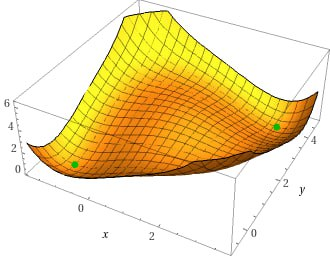
\includegraphics[width=0.5\textwidth]{CorrelationError}
		\label{fig:fig5}
	\end{center}
	\caption{Вид функции $||\hat{\mathbf{\Sigma}}_{t+1} - \bar{\mathbf{\Sigma}}_{t+1}||_2^2$ для двух рядов: $(1, 3)$ и $(2, 4)$. Точки минимума: (3; 4)~--- искомая и (-1; 0)~--- альтернативная}
\end{figure}


Проблемой данного метода является вычислительная затратность методов невыпуклой оптимизации. В качестве альтернативы предлагается следующий метод, использующий только лишь сингулярное разложение матрицы.

\textbf{Теорема 3. (Быстрый метод получения пары возможных ответов.)} \textit{Минимум функции $||\hat{\mathbf{\Sigma}}_{t+1} - \bar{\mathbf{\Sigma}}_{t+1}||_2^2$ достигается на \[\pm\sqrt{\lambda_1} \mathbf{u}_1 + \boldsymbol{\mu}_t,\] где $\lambda_1$--- первое сингулярное значение, $\mathbf{u}_1$--- первый левый сигнулярный вектор матрицы $\mathbf{A}=\left(\hat{\mathbf{\Sigma}}_{t+1} - \frac{t}{t+1} \cdot \mathbf{\Sigma}_t \right) \cdot \frac{(t+1)^2}{t}$}

\textbf{Доказательство.}
Ниже используется обозначение $\mathbf{x}_i$~--- значение \textit{многомерного} временного ряда в момент времени $i$. В доказательстве выражается $\mathbf{\Sigma}_{t+1}$ через $\mathbf{\Sigma}_t$. После чего, используется свойство операторной нормы и ранга матрицы. Все приведенные ниже выражения верны для произвольных $\boldsymbol{\mu}_T$ и $\mathbf{\Sigma}_T$, построенных по определению выше.
\begin{enumerate}
	\item Выразим $\boldsymbol{\mu}$ через значения ряда: \[\boldsymbol{\mu}_t = \frac{1}{t} \sum_{i=1}^{t} \mathbf{x}_i \Rightarrow \sum_{i=1}^{t} \mathbf{x}_i = t \boldsymbol{\mu}_t.\]
	\item Аналогично выразим $\mathbf{\Sigma_t}$ через значения ряда:
		\begin{gather*}
		\mathbf{\Sigma}_t = \frac{1}{t} \sum_{i=1}^{t} (\mathbf{x}_i-\boldsymbol{\mu}_t)(\mathbf{x}_i-\boldsymbol{\mu}_t)^\intercal;\\
		\mathbf{\Sigma}_t = \frac{1}{t} \sum_{i=1}^{t} \mathbf{x}_i \mathbf{x}_i^\intercal - \frac{1}{t} \left( \sum_{i=1}^{t} \mathbf{x}_i\right) \boldsymbol{\mu}_t^\intercal - \boldsymbol{\mu}_t \frac{1}{t} \left( \sum_{i=1}^{t} \mathbf{x}_i^\intercal\right) + \boldsymbol{\mu}_t \boldsymbol{\mu}_t^\intercal = \frac{1}{t} \sum_{i=1}^{t} \mathbf{x}_i \mathbf{x}_i^\intercal - \boldsymbol{\mu}_t \boldsymbol{\mu}_t^\intercal \Rightarrow\\
		\sum_{i=1}^{t} \mathbf{x}_i \mathbf{x}_i^\intercal = t \mathbf{\Sigma}_t + t \boldsymbol{\mu}_t \boldsymbol{\mu}_t^\intercal.
		\end{gather*}
	\item Выразим $\mathbf{\Sigma_{t+1}}$ через $\mathbf{\Sigma_t}$, используя предыдущие выражения:
	\begin{gather*}
		\mathbf{\Sigma}_{t+1} = \frac{1}{t+1} \left(\sum_{i=1}^{t} \mathbf{x}_i \mathbf{x}_i^\intercal + \mathbf{x}_{t+1} \mathbf{x}_{t+1}^\intercal \right) - \boldsymbol{\mu}_{t+1} \boldsymbol{\mu}_{t+1}^\intercal = \\
		= \frac{t}{t+1}\mathbf{\Sigma}_t + \frac{t}{t+1}\boldsymbol{\mu}_{t} \boldsymbol{\mu}_{t}^\intercal + \frac{1}{t+1} \mathbf{x}_{t+1} \mathbf{x}_{t+1}^\intercal - \frac{1}{(t+1)^2} (t \boldsymbol{\mu}_t + \mathbf{x}_{t+1})(t \boldsymbol{\mu}_t + \mathbf{x}_{t+1})^\intercal =\\
		= \frac{t}{t+1}\mathbf{\Sigma}_t + \frac{t}{t+1}\boldsymbol{\mu}_{t} \boldsymbol{\mu}_{t}^\intercal + \frac{t}{(t+1)^2} \mathbf{x}_{t+1} \mathbf{x}_{t+1}^\intercal - \frac{t^2}{(t+1)^2}\boldsymbol{\mu}_{t} \boldsymbol{\mu}_{t}^\intercal - \frac{t}{(t+1)^2}\boldsymbol{\mu}_{t} \mathbf{x}_{t+1}^\intercal - \frac{t}{(t+1)^2}\mathbf{x}_{t+1} \boldsymbol{\mu}_{t}^\intercal =\\
		= \frac{t}{t+1}\mathbf{\Sigma}_t + \frac{t}{t+1}\boldsymbol{\mu}_{t} \boldsymbol{\mu}_{t}^\intercal - \frac{t}{(t+1)^2} \left( -\mathbf{x}_{t+1} \mathbf{x}_{t+1}^\intercal + t\boldsymbol{\mu}_{t} \boldsymbol{\mu}_{t}^\intercal + \boldsymbol{\mu}_{t} \mathbf{x}_{t+1}^\intercal + \mathbf{x}_{t+1} \boldsymbol{\mu}_{t}^\intercal \right) =\\
		= \frac{t}{t+1}\mathbf{\Sigma}_t + \frac{t}{t+1}\boldsymbol{\mu}_{t} \boldsymbol{\mu}_{t}^\intercal - \frac{t}{(t+1)^2} \left( -(\mathbf{x}_{t+1}-\boldsymbol{\mu}_t)(\mathbf{x}_{t+1}-\boldsymbol{\mu}_t)^\intercal + (t+1)\boldsymbol{\mu}_{t} \boldsymbol{\mu}_{t}^\intercal \right) =\\
		= \frac{t}{t+1}\mathbf{\Sigma}_t + \frac{t}{t+1}\boldsymbol{\mu}_{t} \boldsymbol{\mu}_{t}^\intercal - \frac{t(t+1)}{(t+1)^2}\boldsymbol{\mu}_{t} \boldsymbol{\mu}_{t}^\intercal + \frac{t}{(t+1)^2}(\mathbf{x}_{t+1}-\boldsymbol{\mu}_t)(\mathbf{x}_{t+1}-\boldsymbol{\mu}_t)^\intercal =\\
		= \frac{t}{t+1}\mathbf{\Sigma}_t + \frac{t}{(t+1)^2}(\mathbf{x}_{t+1}-\boldsymbol{\mu}_t)(\mathbf{x}_{t+1}-\boldsymbol{\mu}_t)^\intercal.
	\end{gather*}
	Данное равенство выражает $\mathbf{\Sigma}_{t+1}$ через $\mathbf{\Sigma}_t$. Для дальнейшего доказательства полезно вывести следующее равенство для нашей задачи: \[(\bar{\mathbf{x}}_{t+1}-\boldsymbol{\mu}_t)(\bar{\mathbf{x}}_{t+1}-\boldsymbol{\mu}_t)^\intercal = \left(\bar{\mathbf{\Sigma}}_{t+1} - \frac{t}{t+1} \cdot \mathbf{\Sigma}_t \right) \cdot \frac{(t+1)^2}{t}.\]
	
	\item Решается задача поиска минимума функции $||\hat{\mathbf{\Sigma}}_{t+1} - \bar{\mathbf{\Sigma}}_{t+1}||_2^2$. В нашем случае это аналогично равенству этой функции нулю. Распишем выражение под нормой:
	\begin{gather*}
		\hat{\mathbf{\Sigma}}_{t+1} - \bar{\mathbf{\Sigma}}_{t+1} = \frac{t}{t+1}\mathbf{\Sigma}_t + \frac{t}{(t+1)^2}(\hat{\mathbf{x}}_{t+1}-\boldsymbol{\mu}_t)(\hat{\mathbf{x}}_{t+1}-\boldsymbol{\mu}_t)^\intercal - \frac{t}{t+1}\mathbf{\Sigma}_t + \frac{t}{(t+1)^2}(\bar{\mathbf{x}}_{t+1}-\boldsymbol{\mu}_t)(\bar{\mathbf{x}}_{t+1}-\boldsymbol{\mu}_t)^\intercal =\\
		=\frac{t}{(t+1)^2}(\hat{\mathbf{x}}_{t+1}-\boldsymbol{\mu}_t)(\hat{\mathbf{x}}_{t+1}-\boldsymbol{\mu}_t)^\intercal -\frac{t}{(t+1)^2}(\bar{\mathbf{x}}_{t+1}-\boldsymbol{\mu}_t)(\bar{\mathbf{x}}_{t+1}-\boldsymbol{\mu}_t)^\intercal.
 	\end{gather*}
 	Тогда, задача выше эквивалентна нахождению минимума функции \[||(\hat{\mathbf{x}}_{t+1}-\boldsymbol{\mu}_t)(\hat{\mathbf{x}}_{t+1}-\boldsymbol{\mu}_t)^\intercal-(\bar{\mathbf{x}}_{t+1}-\boldsymbol{\mu}_t)(\bar{\mathbf{x}}_{t+1}-\boldsymbol{\mu}_t)^\intercal||_2^2.\]
 	Обозначим \[\mathbf{A} = (\bar{\mathbf{x}}_{t+1}-\boldsymbol{\mu}_t)(\bar{\mathbf{x}}_{t+1}-\boldsymbol{\mu}_t)^\intercal = \left(\bar{\mathbf{\Sigma}}_{t+1} - \frac{t}{t+1} \cdot \mathbf{\Sigma}_t \right) \cdot \frac{(t+1)^2}{t}.\]
 	Ранг матрицы ($\hat{\mathbf{x}}_{t+1}-\boldsymbol{\mu}_t)(\hat{\mathbf{x}}_{t+1}-\boldsymbol{\mu}_t)^\intercal$ равен 1, а поскольку искомый минимум равен 0, получается, что и ранг матрицы $\mathbf{A}$ будет равен 1.
 	
 	\item Из прошлого пункта, матрица $\mathbf{A}$ имеет ранг 1. Распишем сингулярное разложение. \[
 		\mathbf{A} = \sum_{i=1}^{1} \lambda_i \mathbf{u}_i \mathbf{v}_i^\intercal = \lambda_1 \mathbf{u}_1 \mathbf{v}_1^\intercal.
 	\]
 	С другой стороны, $\mathbf{A} = (\bar{\mathbf{x}}_{t+1}-\boldsymbol{\mu}_t)(\bar{\mathbf{x}}_{t+1}-\boldsymbol{\mu}_t)^\intercal$. Тогда, \[
 	\bar{\mathbf{x}}_{t+1}-\boldsymbol{\mu}_t = \pm\sqrt{\lambda_1} \mathbf{u}_1 \Leftrightarrow\\
 	\bar{\mathbf{x}}_{t+1} = \pm\sqrt{\lambda_1} \mathbf{u}_1 + \boldsymbol{\mu}_t.
 	\]
 	Знак $\pm$ возникает из того, что в случае симметричной матрицы, имеют место два сингулярных разложения: $\mathbf{A}=\mathbf{U}\mathbf{\Sigma} \mathbf{V}^\intercal=(-\mathbf{U})\mathbf{\Sigma} (-\mathbf{V})^\intercal$.
 	$$ \blacksquare $$
\end{enumerate}

Эта теорема позволяет находить оба минимума функции намного быстрее, чем при использовании стандартных методов оптимизации.

\section{Алгоритм восстановления значений ряда при точном прогнозе матрицы}

Теоремы 2 и 3 показывают, что использование одной матрицы попарных корреляций и информации о первых $t$ моментах времени позволяет получить \textbf{пару} возможных значений после восстановления. В данной секции предлагается метод выбора истинного значения из полученной пары \textit{в случае, если матрица}  $\mathbf{\Sigma}_{t+1}$  \textit{спрогнозирована точно}.

Алгоритм описанный ниже основан на использовании \textbf{двух} спрогнозированных матриц, отвечающих разным подотрезкам времени. Выбирается два различных значения $T, T'$. Прогнозируются две матрицы:
\begin{itemize}
	\item $\mathbf{\Sigma}_{t+1}^1$~--- матрица попарной корреляции для многомерного временного ряда $\mathbf{x}$ на моментах времени от $t-T+2$ до $t+1$ (суммарно $T$ значений).
	\item $\mathbf{\Sigma}_{t+1}^2$~--- матрица попарной корреляции для многомерного временного ряда $\mathbf{x}$ на моментах времени от $t-T'+2$ до $t+1$ (суммарно $T'$ значений).
\end{itemize}

То есть, при восстановлении ответов из этих матриц мы получим две пары ответов, каждый из которых является кандидатом на истинный. При этом, в каждой из пар существует истинный ответ. Предлагается взять ответ из пересечения.

Итоговая схема алгоритма:

\begin{enumerate}
	\item Зафиксируем $T$ и $T': T \neq T'$.
	\item Для $T$ и $T'$ произведем полученный выше алгоритм и получим наборы ответов: \[ [\hat{\mathbf{x}}_{t+1}^1, \hat{\mathbf{x}'}_{t+1}^1], [\hat{\mathbf{x}}_{t+1}^2, \hat{\mathbf{x}'}_{t+1}^2].\]
	\item Найдём тот ответ, который лежит в пересечении.
	В реальный данных вероятность совпадения множеств ответов равна 0, так же как и на синтетических данных с добавлением случайного шума.
\end{enumerate}


\begin{figure}[H]
	\centering
	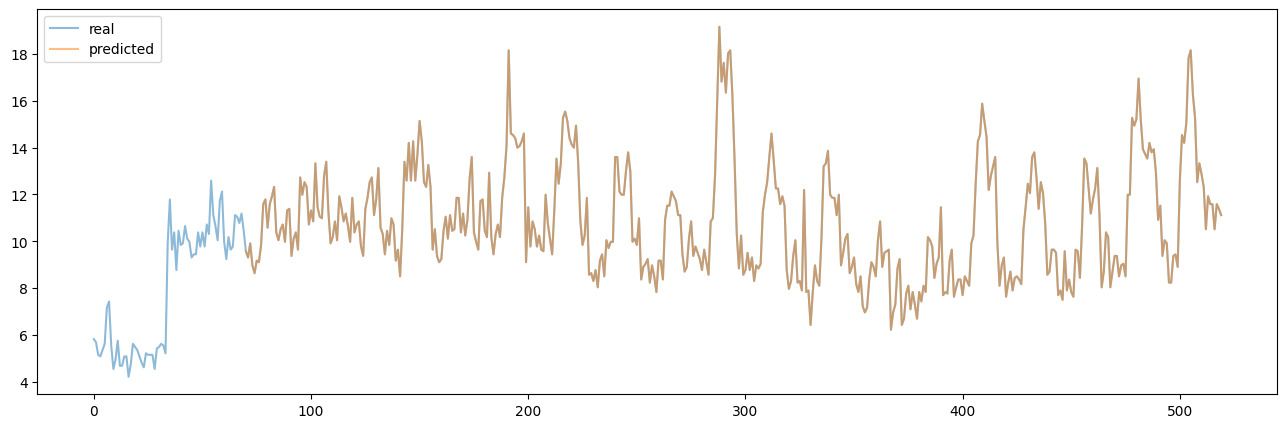
\includegraphics[width=\textwidth]{TwoTAlgo.jpg}
	\caption{Возвращение прогноза при точном прогнозе $\mathbf{\Sigma}$. $T=20$, $T'=10$}
	\label{fig:fig3}
\end{figure}

\section{Алгоритм восстановления значений ряда при неточном прогнозе матрицы}

Проблема вышеописанного алгоритма заключается в том, что при неточном прогнозе, пересечения может не быть. Происходит это из-за того, что ошибка в каждой из спрогнозированных матриц разная. Для этого предлагается следующий алгоритм, амортизирующий ошибку:

Вместо двух значений  $T$ и $T'$ берётся $K$ значений.

Далее, каждая матрица приводится к ближайшей положительной полуопределённой.

Тогда мы молучим $K$ наборов ответов:

\begin{gather*}
	[\hat{\mathbf{x}}_{t+1}^1, \hat{\mathbf{x}'}_{t+1}^1],\\
	[\hat{\mathbf{x}}_{t+1}^2, \hat{\mathbf{x}'}_{t+1}^2],\\
	\vdots \\
	[\hat{\mathbf{x}}_{t+1}^K, \hat{\mathbf{x}'}_{t+1}^K].
\end{gather*}

Далее предлагается перебрать $2^K$ наборов ответов и выбрать тот набор, в котором диаметр минимален. Диаметром называется максимальное евклидово между двумя различными ответами. Это является \textbf{необходимым} условием истинного ответа, то есть такого, который является пересечением всех пар ответов. В случае точного прогноза, диаметр такого набора всегда будет равен нулю.

Асимптотическая сложность данного восстановления будет $O(2^K \times K \times N)$ + сложность используемого алгоритма поиска минимума.

\begin{figure}[H]
	\centering
	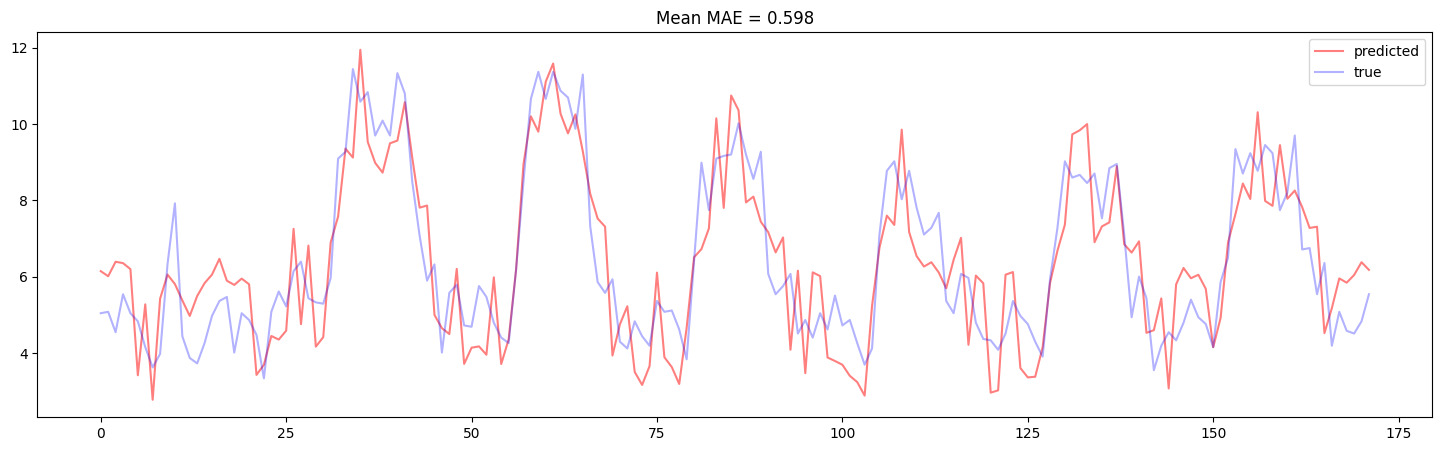
\includegraphics[width=\textwidth]{TbiLSTM.jpg}
	\caption{Возвращение прогноза при неточном прогнозе $\mathbf{\Sigma}$}
	\label{fig:fig4}
\end{figure}

\section{Вычислительный эксперимент}

В данной секции тестируется алгоритм при неточном прогнозе матрицы попарной корреляции из предыдущей секции. Эксперименты проводятся на синтетических данных, а так же на данных температуры трансформатора Electricity Transformer Temperature \cite{zhou2021informer}. Тестируются разные значения $K$, а так же разные добавленные шумы в истинные значения матриц.

\paragraph{Синтетические данные.}\

На таблице ниже приведены значения ошибки после восстановления при разных условиях. Используются сгенерированные данные состоящие из комбинации зашумлённых синусов и косинусов.

\def\arraystretch{2.3}
\begin{tabular}{|l||l||*{3}{c|}}\hline
	\backslashbox{Шум}{Параметры}
	&\makebox[3em]{Метрика}&\makebox[3em]{$K=2$}&\makebox[3em]{$K=4$}&\makebox[3em]{$K=10$}\\\hline
	$\mathcal{N}(0, 0.01)$&\makecell{ MAE: \\ MSE: } &\makecell{ 0.070 \\ 0.010 }&\makecell{ 0.052 \\ 0.005 }&\makecell{ 0.040 \\ 0.002 }\\\hline
	$\mathcal{N}(0, 0.05)$&\makecell{ MAE: \\ MSE: } &\makecell{ 0.316 \\ 0.295 }&\makecell{ 0.176 \\ 0.060 }&\makecell{ 0.116 \\ 0.025 }\\\hline
	$\mathcal{N}(0, 0.1)$& \makecell{ MAE: \\ MSE: } &\makecell{ 0.530 \\ 0.635 }&\makecell{ 0.398 \\ 0.348 }&\makecell{ 0.230 \\ 0.111 }\\\hline
\end{tabular}


\begin{figure}[H]
	\centering
	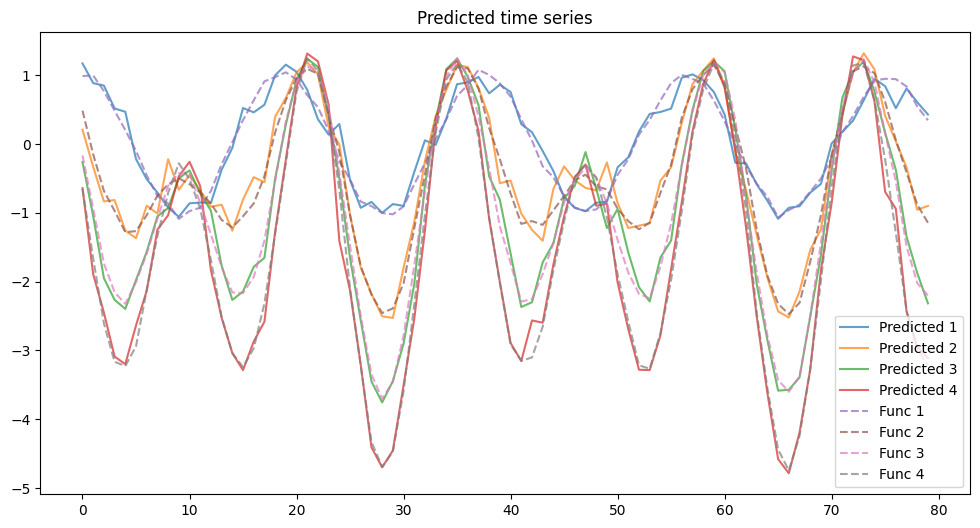
\includegraphics[width=\textwidth]{K10N005.jpg}
	\caption{График восстановления синтетических данных при $K=10$, Добавочный шум $\mathcal{N}(0, 0.05)$. \textbf{MAE: 0.116, MSE: 0.025}}
	\label{fig:fig6}
\end{figure}

\paragraph{Температура электрогенератора.}\

Ниже приведена аналогичная таблица для датасета Electricity Transformer Temperature.

\begin{figure}[H]
	\centering
	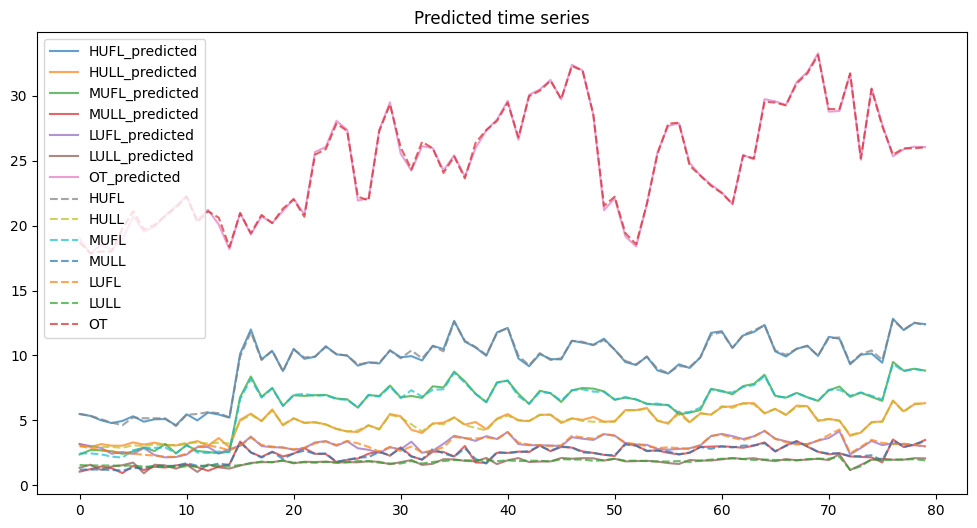
\includegraphics[width=\textwidth]{K10N005_electicity.jpg}
	\caption{График восстановления данных ETTh1 при $K=10$, Добавочный шум $\mathcal{N}(0, 0.05)$. \textbf{MAE: 0.096, MSE: 0.019}}
	\label{fig:fig7}
\end{figure}

\def\arraystretch{2.3}
\begin{tabular}{|l||l||*{3}{c|}}\hline
	\backslashbox{Шум}{Параметры}
	&\makebox[3em]{Метрика}&\makebox[3em]{$K=2$}&\makebox[3em]{$K=4$}&\makebox[3em]{$K=10$}\\\hline
	$\mathcal{N}(0, 0.01)$&\makecell{ MAE: \\ MSE: } &\makecell{ 0.071 \\ 0.030 }&\makecell{ 0.047 \\ 0.004 }&\makecell{ 0.038 \\ 0.003 }\\\hline
	$\mathcal{N}(0, 0.05)$&\makecell{ MAE: \\ MSE: } &\makecell{ 0.240 \\ 0.198 }&\makecell{ 0.153 \\ 0.053 }&\makecell{ 0.096 \\ 0.019 }\\\hline
	$\mathcal{N}(0, 0.1)$& \makecell{ MAE: \\ MSE: } &\makecell{ 0.466 \\ 0.719 }&\makecell{ 0.306 \\ 0.281 }&\makecell{ 0.217 \\ 0.148 }\\\hline
\end{tabular}


Во всех случаях наибольшую точность предсказуемо давало использование большего количества различных значений $T$. Однако, при $K > 15$ алгоритм становится слишком вычислительно сложным из-за экспоненциальной зависимости от $K$.

\section{Заключение}

В статье исследован подход к прогнозированию временных рядов при помощи матрицы попарной корреляции между рядами. Показано, что использование только одной матрицы приводит к существованию пары возможных ответов~--- значений ряда в следующий момент времени. Выведена явная формула вычисления одного ответа через другой, что позволяет решать задачу при помощи невыпуклой оптимизации. Более того, выведен явный вид пары ответов через сингулярное разложение матрицы попарной корреляции. Предложены два алгоритма выявления нужного ответа из пары возможных. Первый опирается на точный прогноз матрицы попарной корреляции. Второй допускает наличие ошибки в прогнозе, однако он более вычислительно требователен.

\bibliography{references}
\bibliographystyle{plain}


\end{document}